\begin{enumerate}[label=\arabic*.,ref=\theenumi]
%
\item A counter is constructed with three $D$ flip-flops. The input-output pairs are named $\brak{D_0, Q_0}$, $\brak{D_1, Q_1}$, and $\brak{D_2, Q_2}$, where the subscript $0$ denotes the least significant bit. The output sequence is desired to be the Gray-code sequence $000, 001, 011, 010, 110, 111, 101$, and $100$, repeating periodically. Note that the bits are listed in the $Q_2$  $Q_1$  $Q_0$ format. The combinational logic expression for $D_1$ is
\hfill(GATE-EE2021,37)
%
\begin{enumerate}
    \item $Q_2 Q_1 Q_0$
    \item $Q_2 Q_0 + Q_1 \Bar{Q_0}$
    \item $\Bar{Q_2} Q_0 + Q_1 \Bar{Q_0}$
    \item $Q_2 Q_1 + \Bar{Q_2} \Bar{Q_1}$
\end{enumerate}
%
\item The propagation delay of the exclusive- OR(XOR) gate in the circuit in  
	\figref{fig:PropagationDelay}
	is $3$ ns. The propagation delay of all the flip-flops is assumed to be zero. The Clock(clk) frequency provided to the circuit is $500$ MHz.
%
	\begin{figure}[H]
    \centering
    \resizebox{0.75\columnwidth}{!}{%
    \begin{circuitikz} 
\draw (2,1)coordinate (E) -- (4,1)coordinate (F) -- (4,-1)coordinate (G) -- (2,-1)coordinate(H) --(2,1)coordinate(E);
\draw (5,1)coordinate (I) -- (7,1)coordinate (J) -- (7,-1)coordinate (K) -- (5,-1)coordinate (L) -- (5,1)coordinate (I);
\draw (8,1)coordinate (M) -- (10,1)coordinate (N) -- (10,-1)coordinate (O) -- (8,-1)coordinate (P) -- (8,1)coordinate (M);
\draw(0,0) node[xor port] (myxor) {};
\draw (myxor.out) |- ($(E)!0.5!(H)$)--++(0:0)node[right]{$D2$};
\draw  ($(F)!0.5!(G)$)--($(I)!0.5!(L)$)--++(0:0)node[right]{$D1$};
\draw ($(J)!0.5!(K)$)--($(M)!0.5!(P)$)--++(0:0)node[right]{$D0$};
\draw ($(N)!0.5!(O)$)--++(0:2)node[right]{}; 
\draw(1,-2) node[above]{$clk$} |- (9,-2);
\draw ($(H)!0.5!(G)$)node[anchor=south,xshift=6]{}--++(90:-1)--++(0:0)node[left]{};
\draw ($(L)!0.5!(K)$)node[anchor=south,xshift=6]{}--++(90:-1)--++(0:0)node[left]{};
\draw ($(P)!0.5!(O)$)node[anchor=south,xshift=6]{}--++(90:-1)--++(0:0)node[left]{};
\draw(2.8,-1) -- (3,-0.8) -- (3.2,-1);
\draw(5.8,-1) -- (6,-0.8) -- (6.2,-1);
\draw(8.8,-1) -- (9,-0.8) -- (9.2,-1);
\draw(myxor.in 1) --++(90:2)-|(4.5,0); 
\draw(myxor.in 2) --++(-90:4)-|(10.5,0); 
\draw(7.5,0) --(7.5,1.5);
\draw(4.85,1.7)node[right]{$Q2$};
\draw(7.85,1.7)node[right]{$Q1$};
\draw(10.85,-1.7)node[right]{$Q0$};
\end{circuitikz}  

		}
    \caption{Propagation Delay}
	\label{fig:PropagationDelay}
\end{figure}
Starting from the initial value of the flip-flop outputs $Q2Q1Q0 =1 1 1$ with $D2=1$,the minimum number of triggering clock edges after which the flip-flop outputs $Q2Q1Q0$ becomes 1 0 0\emph (in integer) is \line(10,0){15}

\hfill(GATE-EC2021,46)
%
\item The maximum clock frequency in MHz of a 4-stage ripple counter, utilizing flip-flops, with each flip-flop having a propagation delay of 20 ns, is \rule{1cm}{0.10mm}. (round off to one decimal place)
\label{gate-ee-2022-29}
\hfill (GATE EE 2022)
%
\item The digital circuit shown 
in \figref{fig:GATE IN 2022-1}
%
	\begin{figure}[H]
    \centering
    \resizebox{0.75\columnwidth}{!}{%
\begin{tikzpicture}
\ctikzset{                                   
logic ports=ieee, 
logic ports/scale=0.5               
}                                    
\draw(-1.3,-0.56)node[nor port,anchor=out](x) {};  
%Drawing flip-flops
\draw (-1.3,-1.3) rectangle (0,0);
\draw(-1,-0.6) node{$D$};
\draw(-2,-1.1) node{$D_0$};
\draw(-0.2,-0.6) node{$Q$};
\draw(0.7,-1.3) rectangle (2,0);
\draw(1,-0.6) node{$D$};
\draw(1.8,-0.6) node{$Q$};
\draw(2.7,-1.3) rectangle (4,0);
\draw(3,-0.6) node{$D$};
\draw(3.8,-0.6) node{$Q$};
%connecting them
\draw(0,-0.6) -- (0.7,-0.6);
\draw(2,-0.6) -- (2.7,-0.6);
\draw(4,-0.6) -- (4.35,-0.6);
%drawing clk
\draw(-1.5,-2) node[above]{$CLK$} -- (3.35,-2);
%connecting clk 
\draw(-0.65,-2) -- (-0.65,-1.3);
\draw(1.35,-2) -- (1.35,-1.3);
\draw(3.35,-2) -- (3.35,-1.3);
\draw(3.35,-2) -- (4,-2);
%drawing clk edges
\draw(-0.5,-1.3) -- (-0.65,-1.1) -- (-0.8,-1.3);
\draw(1.2,-1.3) -- (1.35,-1.1) -- (1.5,-1.3);
\draw(3.2,-1.3) -- (3.35,-1.1) -- (3.5,-1.3);
%drawing Q2,Q1,Q0
%\draw(0.35,-0.6) --(0.35,0.2);
\draw(2.35,-0.6) --(2.35,0.3);
\draw(4.35,-0.6) --(4.35,0.9);
\draw(4.35,0.9) -- (-3,0.9);
\draw(2.35,0.3) -- (-2.5,0.3);
\draw(x.in 2) -|(-3,-0.7)to[short](-3,0.9);
\draw(x.in 1) -|(-2.5,-0.3)to[short](-2.5,0.3);
\draw(0.35,-0.3)node{$Q0$};
\draw(2.35,-0.35)node{$Q1$};
\draw(4.6,-0.35)node{$Q2$};
\end{tikzpicture}
	}
    \caption{}
	\label{fig:GATE IN 2022-1}
\end{figure}
\begin{enumerate}[label=(\Alph*)]
    \item is a divide-by-5 counter
    \item is a divide-by-7 counter
    \item is a divide-by-8 counter
    \item does not function as a counter due to disjoint cycles of states 
\end{enumerate}
\hfill{GATE IN 2022}
\item The propogation delay of the exclusive-OR(XOR) gate in the circuit in 
	\figref{fig:GATE EC 2021}
	is 3ns. The propogation delay of all the flip-flops is assumed to be zero. The clock(Clk) frequency provided to the circuit is 500MHz.
\label{prob:gate-ec-46.2021}

\hfill (GATE EC 2021)
%
	\begin{figure}[H]
    \centering
    \resizebox{0.75\columnwidth}{!}{%
\begin{tikzpicture}
\ctikzset{                                   
logic ports=ieee,                   
logic ports/scale=0.5               
}                                    
\draw(-1.3,-0.56)node[xor port,anchor=out](x) {};  
%Drawing flip-flops
\draw (-1.3,-1.3) rectangle (0,0);
\draw(-1,-0.6) node{$D2$};
\draw(0.7,-1.3) rectangle (2,0);
\draw(1,-0.6) node{$D1$};
\draw(2.7,-1.3) rectangle (4,0);
\draw(3,-0.6) node{$D0$};
%connecting them
\draw(0,-0.6) -- (0.7,-0.6);
\draw(2,-0.6) -- (2.7,-0.6);
\draw(4,-0.6) -- (4.35,-0.6);
%drawing clk
\draw(-1.5,-2) node[above]{$clk$} -- (3.35,-2);
%connecting clk 
\draw(-0.65,-2) -- (-0.65,-1.3);
\draw(1.35,-2) -- (1.35,-1.3);
\draw(3.35,-2) -- (3.35,-1.3);
%drawing clk edges
\draw(-0.5,-1.3) -- (-0.65,-1.1) -- (-0.8,-1.3);
\draw(1.2,-1.3) -- (1.35,-1.1) -- (1.5,-1.3);
\draw(3.2,-1.3) -- (3.35,-1.1) -- (3.5,-1.3);
%drawing Q2,Q1,Q0
\draw(0.35,-0.6) --(0.35,0.3);
\draw(2.35,-0.6) --(2.35,0.35);
\draw(4.35,-0.6) --(4.35,0.9);
\draw(4.35,0.9) -- (-3,0.9);
\draw(0.35,0.3) -- (-2.5,0.3);
\draw(x.in 2) -|(-3,-0.7)to[short](-3,0.9);
\draw(x.in 1) -|(-2.5,-0.3)to[short](-2.5,0.3);
\draw(0.35,0.5)node{$Q2$};
\draw(2.35,0.45)node{$Q1$};
\draw(4.35,1)node{$Q0$};
\end{tikzpicture}
	}
    \caption{}
	\label{fig:GATE EC 2021}
\end{figure}

Starting from the initial value of the flip-flop outputs $Q2Q1Q0 =111$ with $D2=1$,the minimum number of triggering clock edges after which the flip-flop outputs $Q2Q1Q0$ becomes 1 0 0\emph{(in integer)} is \line(1,0){12.5} 

\item  
\label{prob:gate IN 17}
For the $3$-bit binary counter shown in 
\figref{fig:lcd}, the output increments at every positive 
transition in the clock (CLK). Assume ideal diodes and the starting state of the counter as 
$000$. If output high is $1 V$ and output low is $0 V$, the current $I$(in mA) flowing through the 
$50 \Omega$ resistor during the $5$th clock cycle is (up to one decimal place)
\hfill(GATE IN 2018)
\begin{figure}[H]
\centering
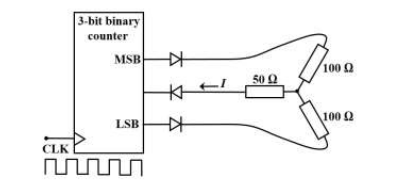
\includegraphics[width=0.75\columnwidth]{ide/7474/figs/pic.png}
\caption{}
\label{fig:lcd}
\end{figure}
\item
\label{prob:gate CS 22}
Consider the sequential circuit shown in \figref{fig:wert}, where both flip-flops used are positive
    edge-triggered D flip-flops.
\begin{figure}[H]
        \centering      
        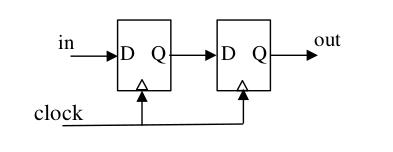
\includegraphics[width=0.75\columnwidth]{ide/7474/figs/wert.jpg}
        \caption{}    
        \label{fig:wert}
    \end{figure}
%
The number of states in the state transition diagram of this circuit that have a transition back to the same state on some value of ''in'' is \rule{30pt}{1pt}.
   \hfill(GATE IN 2018)
   \item The synchronous sequential circuit shown below 
in \figref{fig:gate EC 2023}
	   works at a clock frequency of $1 GHz$. The throughput, in $Mbits/s$,and the latency, in $ns$, respectively, are 
	\begin{figure}[H]
    \centering
    \resizebox{0.75\columnwidth}{!}{%
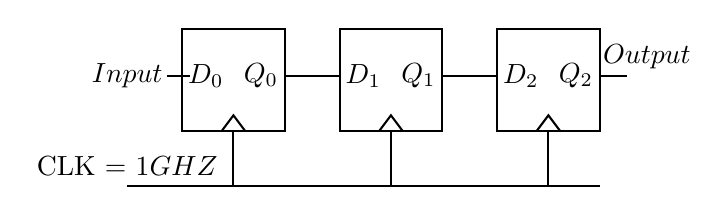
\begin{tikzpicture}
\ctikzset{                                  
    logic ports=ieee,                   
    logic ports/scale=0.5               
}                                    
%
% Drawing flip-flops
\draw (-1.3,-1.3) rectangle (0,0);
\draw(-1,-0.6) node{$D_0$};
\draw(-0.3,-0.6) node{$Q_0$};
\draw(0.7,-1.3) rectangle (2,0);
\draw(1,-0.6) node{$D_1$};
\draw(1.7,-0.6) node{$Q_1$};
\draw(2.7,-1.3) rectangle (4,0);
\draw(3,-0.6) node{$D_2$};
\draw(3.7,-0.6) node{$Q_2$};

% Connecting them
\draw(0,-0.6) -- (0.7,-0.6);
\draw(2,-0.6) -- (2.7,-0.6);
\draw(4,-0.6) -- (4.35,-0.6);
\draw(-1.2,-0.6) -- (-1.5,-0.6);

% Drawing clk
\draw(-2,-2) node[above]{CLK = $1GHZ$ } -- (3.35,-2);

% Connecting clk
\draw(-0.65,-2) -- (-0.65,-1.3);
\draw(1.35,-2) -- (1.35,-1.3);
\draw(3.35,-2) -- (3.35,-1.3);
\draw(3.35,-2) -- (4,-2);

% Drawing clk edges
\draw(-0.5,-1.3) -- (-0.65,-1.1) -- (-0.8,-1.3);
\draw(1.2,-1.3) -- (1.35,-1.1) -- (1.5,-1.3);
\draw(3.2,-1.3) -- (3.35,-1.1) -- (3.5,-1.3);

% Drawing Q2, Q1, Q0
\draw(0.35,-0.3)node{};
\draw(2.35,-0.35)node{};
\draw(4.6,-0.35)node{$ Output $};
\draw(-2,-0.6)node{$ Input $};
\end{tikzpicture}
	}
		\caption{}
\label{fig:gate EC 2023}
\end{figure}

    \begin{enumerate}
        \item $1000, 3$
         \item $333.33, 1$
          \item $2000, 3$
           \item $333.33 , 3$
    \end{enumerate}
\hfill(GATE EC 2023)
\label{prob:GATE EC 2023}
\item In a given sequential circuit
	in \figref{fig:GATE EC 2023},
	 initial states are $Q1 = 1$ and $Q2 = 0$. For a clock frequency of $1 MHz$, the frequency of signal $Q2$ in kHz, is(rounded off to the nearest integer)
   % 
	\begin{figure}[H]
    \centering
    \resizebox{0.75\columnwidth}{!}{%
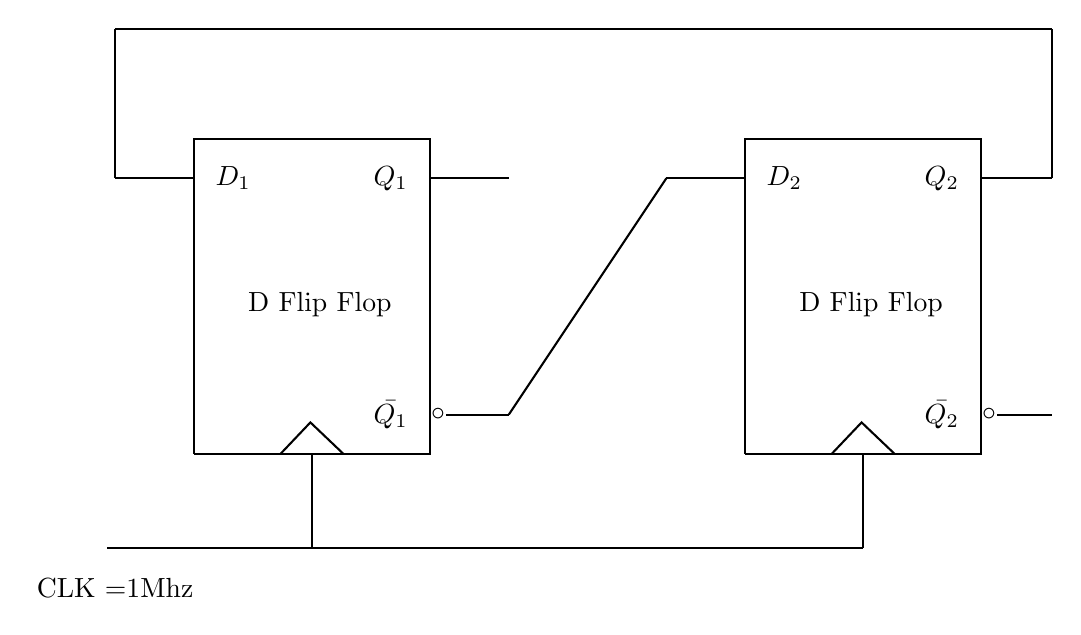
\begin{tikzpicture}              

%Drawing flip-flops
\draw (1.6,1.9) node {D Flip Flop};
\draw (0,0)--(3,0)--(3,4)--(0,4)--(0,0);
\draw(0.5,3.5) node{$D_1$};
\draw(2.5,3.5) node{$Q_1$};
\draw(2.5,0.5) node{$\bar{Q_1}$};
\draw(3.1,0.5) node{$\circ$};

\draw (8.6,1.9) node {D Flip Flop};
\draw(7,0)--(7,4)--(10,4)--(10,0)--(7,0);
\draw(7.5,3.5) node{$D_2$};
\draw(9.5,3.5) node{$Q_2$};
\draw(9.5,0.5) node{$\bar{Q_2}$};
\draw(10.1,0.5) node{$\circ$};

%connecting them
\draw(3.2,0.5)--(4.0,0.5);
\draw(10.2,0.5)--(10.9,0.5);
\draw(7.0,3.5)--(6.0,3.5);
\draw(4.0,0.5) -- (6.0,3.5);
\draw(10.0,3.5) -- (10.9,3.5);
\draw(4.0,3.5) --(3.0,3.5);

\draw(-1.1,-1.2)-- (8.5,-1.2);

%drawing clk
\draw (-1.0,-1.7)node{CLK =1Mhz};


%connecting clk 
\draw(1.5,-1.2) -- (1.5,0.0);
\draw(8.5,-1.2) -- (8.5,0.0);

%drawing clk edges
\draw(1.1,0.0) -- (1.48,0.4) -- (1.9,0.0);
\draw(8.1,0.0) -- (8.48,0.4) -- (8.9,0.0);

% Drawing Q2, D1,
\draw(10.9,3.5)--(10.9,5.4);
\draw(10.9,5.4)--(-1.0,5.4);
\draw(-1.0,5.4)--(-1.0,3.5);
\draw(0,3.5)--(-1.0,3.5);
\end{tikzpicture}
	}
    \caption{}
	\label{fig:GATE EC 2023}
\end{figure}
\hfill(GATE EC 2023)
%
\item Neglecting the delays due to the logic gates in the circuit shown in 
\figref{fig:Gate_question.png},
 the 
decimal equivalent of the binary sequence $[ABCD]$ of initial logic states, which will not change with clock, is $\underline{\hspace{2cm}}$.\\

\hfill{(EE GATE 2023)}\\

\begin{figure}[H]
 \centering
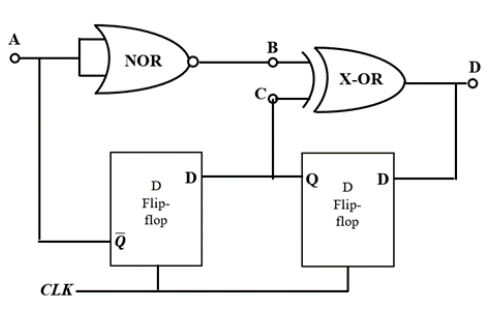
\includegraphics[width=0.75\columnwidth]{ide/7474/figs/Gate_question.png}
\caption{}
\label{fig:Gate_question.png}
\end{figure}

\item 
Consider a sequential digital circuit consisting of T flip-flops and D flip-flops as shown in 
\figref{fig:Flip-Flop}.
 CLKIN is is the clock input to the circuit. At the beginning,Q1,Q2 and Q3 have values 0,1 and 1, respectively.
%
	\begin{figure}[H]
    \centering
    \resizebox{0.75\columnwidth}{!}{%
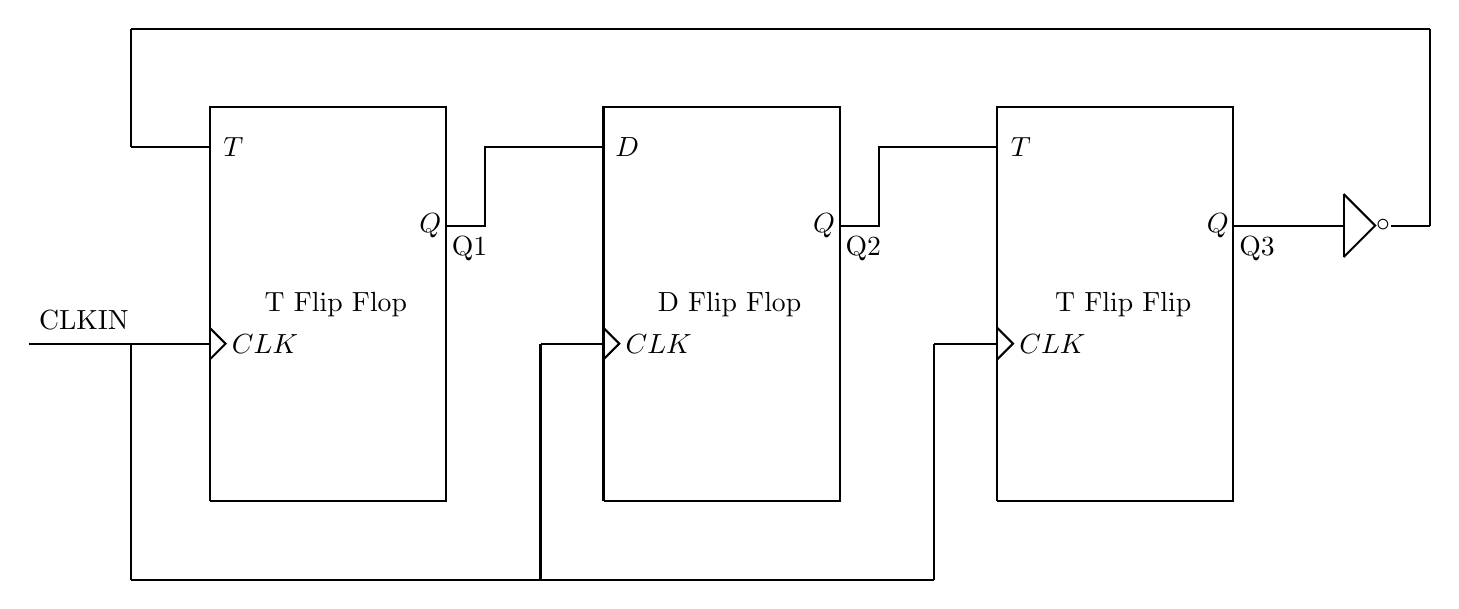
\begin{tikzpicture}      
%Drawing flip-flops
\draw (1.6,2.5) node {T Flip Flop};
\draw (0,0)--(3,0)--(3,5)--(0,5)--(0,0);
\draw(0.3,4.5) node{$T$};
\draw(2.8,3.5) node{$Q$};
\draw(0.7,2.0) node{$CLK$};
\draw (6.6,2.5) node {D Flip Flop};
\draw(5,0)--(5,5)--(8,5)--(8,0)--(5,0);
\draw(5.3,4.5) node{$D$};
\draw(7.8,3.5) node{$Q$};
\draw(5.7,2.0) node{$CLK$};
\draw (11.6,2.5) node {T Flip Flip};
\draw (10,0)--(10,5)--(13,5)--(13,0)--(10,0);
\draw (10.3,4.5) node{$T$};
\draw (12.8,3.5) node{$Q$};
\draw(10.7,2.0) node{$CLK$};
%connecting them
\draw(-1.0,2.0)--(-1.0,-1.0);
\draw(3.0,3.5)--(3.5,3.5)--(3.5,4.5)--(5.0,4.5);
\draw(8.0,3.5)--(8.5,3.5)--(8.5,4.5)--(10.0,4.5);
\draw(9.2,-1.0)--(9.2,2.0);
\draw(4.2,-1.0)--(4.2,2.0);
\draw(-1.0,-1.0)--(9.2,-1.0);
\draw(0.0,4.5)--(-1.0,4.5);
\draw(-1.0,4.5)--(-1.0,6.0);
\draw(-1.0,6.0)--(15.5,6.0);
\draw(14.4,3.1)--(14.4,3.9);
\draw(15.5,6.0)--(15.5,3.5);
\draw(15.5,3.5)--(15.0,3.5);
\draw(14.9,3.5) node{$\circ$};
%drawing clk
\draw (-1.6,2.3)node{CLKIN};
\draw (3.3,3.2)node{Q1};
\draw (8.3,3.2)node{Q2};
\draw (13.3,3.2)node{Q3};
%connecting clk 
\draw(-2.3,2.0) -- (0,2.0);
\draw(4.2,2.0) -- (5.0,2.0);
\draw(9.2,2.0) -- (10.0,2.0);
\draw(13.0,3.5) -- (14.4,3.5);
%drawing clk edges
\draw(0.0,1.8) -- (0.2,2.0) -- (0.0,2.2);
\draw(5.0,1.8) -- (5.2,2.0) -- (5.0,2.2);
\draw(10.0,1.8) -- (10.2,2.0) -- (10.0,2.2);
\draw(14.4,3.1) -- (14.8,3.5) -- (14.4,3.9);
\end{tikzpicture}

		}
\caption{}
\label{fig:Flip-Flop}
\end{figure}
Which of the given values of \((Q_1, Q_2, Q_3)\) can NEVER be obtained with this digital circuit?
\begin{enumerate}
    
    \item ${(0,0,1)}$
    \item ${(1,0,0)}$
    \item ${(1,0,1)}$
    \item ${(1,1,1)}$
\end{enumerate}
\hfill(GATE CS2023,43)
\item In the circuit shifter in 
\figref{fig:cricuit Digram},
the initial binary content of the shift register A $1101$ and that of shift register B is $1010$ The shift registers are positive edge triggered, and the gates have no delay.
when the shift control is high,what will be the binary content of the shift registers $A$ and $B$ after clock pulses?

\hfill{(GATE IN 2023)}

\begin{figure}[H]
\centering
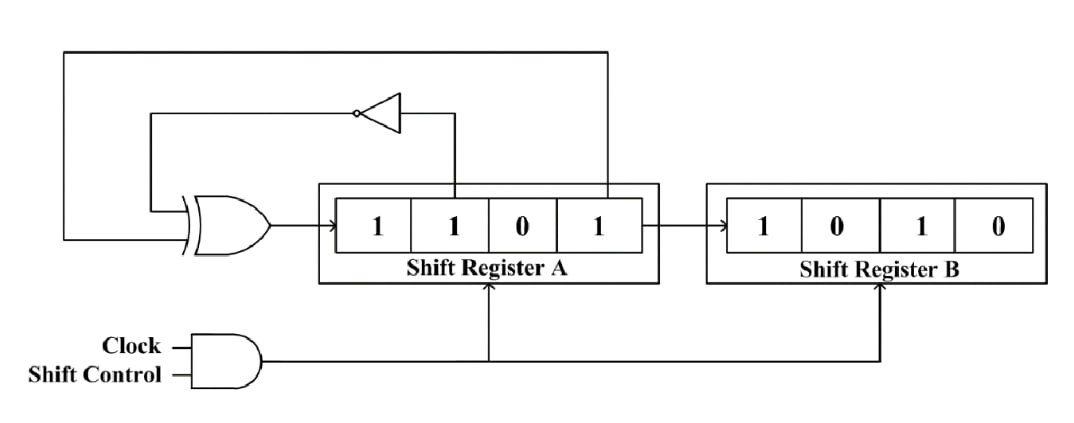
\includegraphics[width=0.75\columnwidth]{ide/7474/figs/Gate.png}
\caption{circuit Digram}
\label{fig:cricuit Digram}
\end{figure}

\begin{enumerate}
\item $A= 1101,B=1101$
\item $A=1110 ,B=1001$
\item $A=0101 ,B=1101$
\item $A=1010 ,B=1111$
\end {enumerate}
\item For the circuit shown
in
			\figref{fig:new_gate},
	 the clock frequency is $f_0$ and the duty cycle is $25\%$. For the signal at the Q output of the Flip-Flop,\hfill(GATE EC 2022)
		\begin{figure}[H]
			\centering
			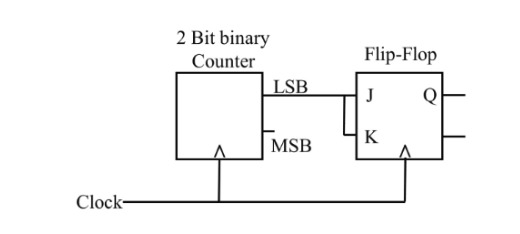
\includegraphics[width=0.75\columnwidth]{ide/7474/figs/gate_image_new.jpg}
			\caption{Circuit}
			\label{fig:new_gate}
		\end{figure}
			\begin{enumerate}
			\item frequency is $\frac{{f_0}}{4}$ and duty cycle is $50\%$
			\item frequency is $\frac{{f_0}}{4}$ and duty cycle is $25\%$
			\item frequency is $\frac{{f_0}}{2}$ and duty cycle is $50\%$
			\item frequency is ${f_0}$ and duty cycle is $25\%$
		\end{enumerate}
\item The digital circuit shown in \figref{fig:GATEIN202236.png}
\begin{figure}[H]
  \centering
  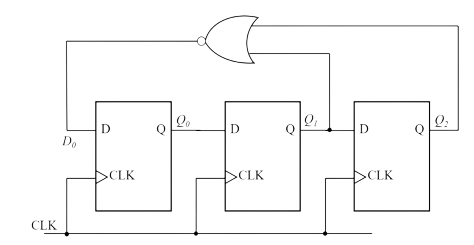
\includegraphics[width=0.75\columnwidth]{ide/7474/figs/GATEIN202236.png}
  \caption{}
  \label{fig:GATEIN202236.png}
\end{figure}
 \begin{enumerate}
 \item is a divide-by-$5$ counter
 \item is a divide-by-$7$ counter
 \item is a divide-by-$8$ counter
 \item does not function as a counter due to disjoint cycles of states 
\end{enumerate}
\hfill(GATE-IN-2022)

 \item Given below 
in
		      \figref{fig:GATE-IN2021}
	 is the diagram of a synchronous sequential circuit with one $J-K$ flip-flop and one $T$ flip-flop with their outputs denoted as $A$ and $B$ respectively, with $J_{A}=\brak{A^{\prime}+B^{\prime}}$, $K_{A}=(A+B)$ and $T_{B}=A$.Starting from the initial state $\brak{AB=00}$, the sequence of states $\brak{AB}$ visited by the circuit is
\hfill(GATE-IN2021)
	\begin{figure}[H]
    \centering
    \resizebox{0.75\columnwidth}{!}{%
		       \begin{circuitikz}
            \draw (2,2)coordinate(w)--(5,2)coordinate(x)--(5,6)coordinate(x)--(2,6)coordinate(z)--(2,2)coordinate(w);
            \draw (1,5.5)--(2,5.5);
           \draw (1,5.8)node[]{$A^{\prime}+B^{\prime}$};
            \draw (2,5.5)node[right]{$J_A$};
            \draw (5,5.5)node[left]{$A$};
            \draw (5,5.5)--(5.5,5.5);
            \draw (1,2.5)--(2,2.5);
            \draw (1,2.8)node[]{$A+B$};
            \draw(2,2.5)node[right]{$K_A$};
            \draw(5,2.5)node[left]{$A^{\prime}$};
           \draw(5,2.5)--(5.5,2.5);
           \draw[->] (0,4)--(2,4);
            \draw (0,4)--(0,0);
            \draw (-1,0)--(7,0);
            \draw (0,0.3)node[left]{$\text{clock}$};
            \draw  (2,4.5)--(2.5,4)--(2,3.5);
            
             \draw (8,2)rectangle(10,6); 
             \draw (8,4.5)--(8.3,4)--(8,3.5);
             \draw (7,5.5)--(8,5.5)node[right]{$T_{B}$};
             \draw (10,5.5)node[left]{$B$}--(10.5,5.5);
             \draw (10,2.5)node[left]{$B^{\prime}$}--(10.5,2.5);
             \draw[->] (7,4)--(8,4);
             \draw (7,4)--(7,0);
            
        \end{circuitikz}

		      }
		      \caption{}
		      \label{fig:GATE-IN2021}
	      \end{figure}
		  \begin{enumerate}
          \item $00 \rightarrow 01 \rightarrow 10 \rightarrow 11 \rightarrow 00 
          \dots $
          \item $00 \rightarrow 10 \rightarrow 01 \rightarrow 11 \rightarrow 00 
          \dots $
          \item $00 \rightarrow 10 \rightarrow 11 \rightarrow 01 \rightarrow 00 \dots $
          \item $00 \rightarrow 01 \rightarrow 11 \rightarrow 00 \dots $
      \end{enumerate}
  \item Consider the $D$-Latch shown in 
	\figref{fig:GATE-EC2017},
		which is transparent when its clock input $CK$ is high and has zero propagation delay. In the figure, the clock signal $CLK1$ has $50\%$ duty cycle and $CLK2$ is a one fifth period delayed version of $CLK1$. The duty cycle at the output of the latch in percentage is \rule{1cm}{1pt}.
  \hfill(GATE-EC2017)
	\begin{figure}[H]
    \centering
    \resizebox{0.75\columnwidth}{!}{%
			      
\begin{tikzpicture}
    \draw[draw=black, thin, solid] (-5.00,0.00) -- (-4.50,0.00);
    \draw[draw=black, thin, solid] (-4.50,0.00) -- (-4.50,0.50);
    \draw[draw=black, thin, solid] (-4.50,0.50) -- (-3.50,0.50);
    \draw[draw=black, thin, solid] (-3.50,0.50) -- (-3.50,0.00);
    \draw[draw=black, thin, solid] (-3.50,0.00) -- (-3.00,0.00);
    \draw[draw=black, thin, solid] (-3.00,0.00) -- (-2.50,0.00);
    \draw[draw=black, thin, solid] (-2.50,0.00) -- (-2.50,0.50);
    \draw[draw=black, thin, solid] (-2.50,0.50) -- (-1.50,0.50);
    \draw[draw=black, thin, solid] (-1.50,0.50) -- (-1.50,0.00);
    \draw[draw=black, thin, solid] (-1.50,0.00) -- (-0.50,0.00);
    \draw[draw=black, thin, solid] (-0.50,0.00) -- (-0.50,0.50);
    \draw[draw=black, thin, solid] (-0.50,0.50) -- (0.00,0.50);
    \draw[draw=black, thin, solid] (-5.00,-1.00) -- (-4.00,-1.00);
    \draw[draw=black, thin, solid] (-4.0,-2.2) -- (-4.0,-1.80);
    \draw[draw=black, thin, solid] (-4.5,-2.2) -- (-4.5,-1.80);
    \draw[draw=black, thin, solid] (-4.5,1.15) -- (-4.5,0.85);
    \draw[draw=black, thin, solid] (-2.5,1.15) -- (-2.5,0.85);
    \draw[draw=black, thin, solid] (-4.00,-1.00) -- (-4.00,-0.50);
    \draw[draw=black, thin, solid] (-4.00,-0.50) -- (-3.00,-0.50);
    \draw[draw=black, thin, solid] (-3.00,-0.50) -- (-3.00,-1.00);
    \draw[draw=black, thin, solid] (-3.00,-1.00) -- (-2.00,-1.00);
    \draw[draw=black, thin, solid] (-2.00,-1.00) -- (-2.00,-0.50);
    \draw[draw=black, thin, solid] (-2.00,-0.50) -- (-1.00,-0.50);
    \draw[draw=black, thin, solid] (-1.00,-0.50) -- (-1.00,-1.00);
    \draw[draw=black, thin, solid] (-1.00,-1.00) -- (0.00,-1.00);
    \draw[draw=black, thin, dotted] (-4.50,0.00) -- (-4.50,-2.00);
    \draw[draw=black, thin, dotted] (-4.00,0.50) -- (-4.00,-2.00);
    \draw[draw=black, -latex, thin, solid] (-5.00,-2.00) -- (-4.50,-2.00);
    \draw[draw=black, -latex, thin, solid] (-3.50,-2.00) -- (-4.00,-2.00);
    \draw[draw=black, latex-, thin, solid] (-4.50,1.00) -- (-3.50,1.00);
    \draw[draw=black, latex-, thin, solid] (-2.50,1.00) -- (-3.00,1.00);
    \draw[draw=black, thin, solid] (1.50,1.00) -- (1.50,-1.00);
    \draw[draw=black, thin, solid] (1.50,-1.00) -- (3.50,-1.00);
    \draw[draw=black, thin, solid] (3.50,1.00) -- (3.50,-1.00);
    \draw[draw=black, thin, solid] (1.50,1.00) -- (3.50,1.00);
    \draw[draw=black, thin, solid] (2.50,-1.00) -- (2.50,-1.50);
    \draw[draw=black, thin, solid] (2.50,-1.50) -- (1.00,-1.50);
    \draw[draw=black, thin, solid] (1.50,0.50) -- (0.50,0.50);
    \draw[draw=black, thin, solid] (3.50,0.50) -- (4.50,0.50);
    \draw[draw=black, thin, solid] (0.50,0.50) circle (0.1);
    \draw[draw=black, thin, solid] (4.50,0.50) circle (0.1);
    \draw[draw=black, thin, solid] (1.00,-1.50) circle (0.1);
    \node[black, anchor=south west] at (-6,0){\footnotesize $CLK1$};
    \node[black, anchor=south west] at (-6,-1) {\footnotesize $CLK2$};
    \node[black, anchor=south west] at (-0.06,0.75){\footnotesize $CLK1$};
    \node[black, anchor=south west] at (-0.06,-2.25) {\footnotesize $CLK2$};
    \node[black, anchor=south west] at (3.94,0.75) {Output};
    \node[black, anchor=south west] at (1.54,0.25) {\footnotesize $D$};
    \node[black, anchor=south west] at (2.84,0.21) {\footnotesize $Q$};
    \node[black, anchor=south west] at (1.80,-0.25) {\footnotesize $D$-latch};
    \node[black, anchor=south west] at (2.05,-1.0) {\footnotesize $CK$};
    \node[black, anchor=south west] at (-4.76,-3.2) {\footnotesize $\dfrac{T_{CLK}}{5}$};
    \node[black, anchor=south west] at (-3.8,1.1) {\footnotesize $T_{CLK}$};
\end{tikzpicture}
	}
    \caption{}
	\label{fig:GATE-EC2017}
\end{figure}
\item A $4$-bit shift register circuit configured for right-shift operation, i.e.\\ $D_{in} \rightarrow A, A \rightarrow B, B \rightarrow C, C \rightarrow D$, is shown
	in \figref{fig:GATE-EC-2017}.
 If the present state of the shift register is $ABCD = 1101$, the number of clock cycles required to reach the state $ABCD = 1111$ is

\hfill (GATE-EC 2017)
	\begin{figure}[H]
    \centering
    \resizebox{0.75\columnwidth}{!}{%
	\begin{circuitikz}
	%nodes
	\draw (-1,0) node[xor port, rotate=180,scale =1.5](xor1) {};
	\draw (2,-3) node[rectangle, scale = 2,draw, outer sep = 0] (a) {A};
	\draw (3,-3) node[rectangle, scale = 2,draw, anchor = west, outer sep = 0] (b) at (a.east) {B};
	\draw (4,-3) node[rectangle, scale = 2,draw, anchor = west, outer sep = 0] (c) at (b.east) {C};
	\draw (5,-3) node[rectangle, scale = 2,draw, anchor = west, outer sep = 0] (d) at (c.east) {D};
        
        %connection
        \draw (xor1.out) to (-2,0)
        (-2,0) to (-2,-2.75)
        (-2,-2.75) to (1.4,-2.75);
        \draw (xor1.in 1) to (2,-0.43)
        (2,-0.43) to (2,-2.45);
        \draw (1.4,-3.25) to (0.25,-3.25);
        \draw (xor1.in 2) to (5.5,0.43)
        (5.5,0.43) to (5.5,-2.45) ;
        
        %naming
        \draw (-1,-2.5) node[rectangle, scale = 1.5]{$\text{D}_{\text{in}}$};
        \draw (0.25,-3.5) node[rectangle, scale = 1.5] {Clock};
        
\end{circuitikz}


		}
 	\caption{}
	\label{fig:GATE-EC-2017}
\end{figure}

\item In the circuit shown
	in \figref{fig:GATE-EC2019,25},
the clock frequency, i.e., the frequency of the clk signal, is 12 KHz. The frequency of the signal at $\mathbf{Q2}$ is $\underline{\hspace{18pt}}$ KHz.
		\hfill(GATE-EC2019,25)
%%\end{enumerate}
	\begin{figure}[H]
    \centering
    \resizebox{0.75\columnwidth}{!}{%
			
\begin{circuitikz}

\draw (7,2)coordinate (E) -- (9,2)coordinate (F) -- (9,-1)coordinate (G) -- (7,-1)coordinate (H) -- (7,2)coordinate (E);
\draw (11,2)coordinate (I) -- (13,2)coordinate (J) -- (13,-1)coordinate (K) -- (11,-1)coordinate (L) -- (11,2)coordinate (I);
% AND Gate
\draw (6,1.5) node[and port] (and) {};
\draw (and.in 1) node[left] {};
\draw (and.in 2) node[left] {};
\draw (and.out) |- ($(E)!0.2!(H)$)--++(0:0)node[right]{$D1$}; % and gate output is connected to d1.

%clock
\draw ($(L)!0.5!(K)$)node[anchor=south]{$clk$};
\draw ($(H)!0.5!(G)$)node[anchor=south]{$clk$};
\draw(6,-2) node[above]{$12 \textsl{KHz}$} |- (12,-2);
\draw ($(H)!0.5!(G)$)node[anchor=south,xshift=6]{}--++(90:-1)--++(0:0)node[left]{};
\draw ($(L)!0.5!(K)$)node[anchor=south,xshift=6]{}--++(90:-1)--++(0:0)node[left]{};

\draw($(F)!0.2!(G)$)node[left]{$Q1$} -- ($(I)!0.2!(L)$)node[right]{$D2$}; % q1 is connected to d2.
    
\draw($(F)!0.8!(G)$)node[left]{$\overline{Q1}$};
    
\draw($(J)!0.2!(K)$)node[left]{$Q2$};
    
\draw($(J)!0.8!(K)$)node[left]{$\overline{Q2}$};
    
    
\draw ($(J)!0.2!(K)$)--++(0:1)node[right]{};
    
\draw(and.in 1) --++(90:2)-|(9.5,1)|-($(F)!0.8!(G)$)(0:0)node[left]{}; % and gate input 1 is connected to q1 bar.
    
\draw(and.in 2) --++(-90:4)-|(13.5,-0.5)|- ($(J)!0.8!(K)$);  % and gate input 2 is connected to q2 bar.
    
\end{circuitikz}

			}
    \caption{}
	\label{fig:GATE-EC2019,25}
\end{figure}
%
 \item The circuit shown in 
	\figref{fig:GATE-IN2019,12}
below uses ideal positive edge-triggered synchronous $J-K$ flip flops with outputs $X$ and $Y$. If the initial state of the output is $X=0$ and $Y=0$ just before the arrival of the first clock pulse, the state of the output just before the arrival of the second clock pulse is
              \hfill(GATE-IN2019,12)
	\begin{figure}[H]
    \centering
    \resizebox{0.75\columnwidth}{!}{%
    \begin{circuitikz}
            \draw (2,2)coordinate(w)--(5,2)coordinate(x)--(5,6)coordinate(x)--(2,6)coordinate(z)--(2,2)coordinate(w);
            \draw (1,5.5)--(2,5.5);
           \draw (1,5.5)node[left]{$1$};
            \draw (2,5.5)node[right]{$J$};
            \draw (5,5.5)node[left]{$Q$};
            \draw (5,5.5)--(5.5,5.5);
            \draw (1,2.5)--(2,2.5);
            \draw (1,2.5)node[left]{$1$};
            \draw(2,2.5)node[right]{$K$};
	   \draw[->] (1,4)--(2,4);
            \draw [->] (5.5,5.5)--(6.5,5.5)--(6.5,4)--(8,4);
	    \draw  (2,4.5)--(2.5,4)node[right]{$CLK$}--(2,3.5);
            
             \draw (8,2)rectangle(11,6); 
             \draw (8,4.5)--(8.5,4)node[right]{$CLK$}--(8,3.5);
             \draw (7.5,5.5)node[left]{$1$}--(8,5.5)node[right]{$J$};
             \draw (11,5.5)node[left]{$Q$}--(11.5,5.5);
	     \draw (7.5,2.5)node[left]{1}--(8,2.5)node[right]{$K$};
             
	     \draw[-o](5.5,5.5)--(5.5,7)--(13,7)--(13,4);
	     \draw[-o] (11.5,5.5)--(12,5.5)--(12,4);
	  \draw(12.5,2.7)node[]{$Output$}; 
             \draw(12,3.5)node[]{$X$};
             \draw (13,3.5)node[]{$Y$};
             \draw (-1.5,3.5)--(-1,3.5)--(-1,4.5)--(-0.5,4.5)--(-0.5,3.5)--(0,3.5)--(0,4.5)--(0.5,4.5)--(0.5,3.5)--(1,3.5);
            
        \end{circuitikz}


	}
    \caption{}
	\label{fig:GATE-IN2019,12}
\end{figure}
%
\begin{enumerate}
    \item $X=0$, $Y=0$
    \item $X=0$, $Y=1$
    \item $X=1$, $Y=0$
    \item$X=1$, $Y=1$
\end{enumerate}

\item Consider a $4$-bit counter constructed out of four flip-flops.It is formed by connecting the J and K inputs to logic high and feeding the Q output to the clock input of the following flip-flop (see 
	\figref{fig:GATE-PH2020,30}
). The input signal to the counter is a series of square pulses and the change of state is triggered by the falling edge.At time t=t0 the outputs are in logic low state (Q0 = Q1 = Q2 = Q3 = 0).Then at t=t1,the logic state of the outputs is 
		               \hfill(GATE-PH2020,30)
\begin{figure}[H]
    \centering
    \resizebox{0.75\columnwidth}{!}{%
\begin{circuitikz}
    \draw (2,2)rectangle(4,6);
    \draw (6,2)rectangle(8,6);
    \draw (10,2)rectangle(12,6);
    \draw (14,2)rectangle(16,6);
    \draw (0,0)node[left]{$1$}--(16,0);
    \draw (0,-0.3)node[right]{$logic~high $};
     \draw (2,5.5)node[right]{$J$}--(1.5,5.5)--(1.5,0);
     \draw (6,5.5)node[right]{$J$}--(5.5,5.5)--(5.5,0);
     \draw (10,5.5)node[right]{$J$}--(9.5,5.5)--(9.5,0);
     \draw (14,5.5)node[right]{$J$}--(13.5,5.5)--(13.5,0);
     \draw (2,2.5)node[right]{$K$}--(1.5,2.5);
     \draw (6,2.5)node[right]{$K$}--(5.5,2.5);
     \draw (10,2.5)node[right]{$K$}--(9.5,2.5);
     \draw (14,2.5)node[right]{$K$}--(13.5,2.5);
     \draw (4,5.5)node[left]{$Q$}--(5,5.5)--(5,4)--(6,4)node[right]{$ck$};
     \draw (8,5.5)node[left]{$Q$}--(9,5.5)--(9,4)--(10,4)node[right]{$ck$};
     \draw (12,5.5)node[left]{$Q$}--(13,5.5)--(13,4)--(14,4)node[right]{$ck$};
     \draw (4.5,5.5)--(4.5,7.5)node[above]{$Q0$};
     \draw (8.5,5.5)--(8.5,7.5)node[above]{$Q1$};
     \draw (12.5,5.5)--(12.5,7.5)node[above]{$Q2$};
     \draw (16,5.5)node[left]{$Q$}--(16.5,5.5)--(16.5,7.5)node[above]{$Q3$};
     \draw (2,4)node[right]{$ck$}--(0.5,4)node[left]{$Input$};
         \draw (4,2.5)node[left]{$\overline{Q}$};
         \draw (8,2.5)node[left]{$\overline{Q}$};
         \draw (12,2.5)node[left]{$\overline{Q}$};
         \draw (16,2.5)node[left]{$\overline{Q}$};
         \draw(4.5,-4)--(5,-4)--(5,-3.5)--(5.5,-3.5)--(5.5,-4)--(6,-4)--(6,-3.5)--(6.5,-3.5)--(6.5,-4)--(7,-4)--(7,-3.5)--(7.5,-3.5)--(7.5,-4)--(8,-4)--(8,-3.5)--(8.5,-3.5)--(8.5,-4)--(9,-4)--(9,-3.5)--(9.5,-3.5)--(9.5,-4)-- (10,-4)--(10,-3.5)--(10.5,-3.5)--(10.5,-4)--(11,-4)--(11,-3.5)--(11.5,-3.5)--(11.5,-4)--(12,-4)--(12,-3.5)--(12.5,-3.5)--(12.5,-4)--(13,-4);
         \draw (8,-1) node[]{$ 4-\textsl{bit ripple counter}$};
         \draw[->] (5.5,-4.5)--(6.5,-4.5)node[right]{$t$};
         \draw (7,-5)node[right]{$\textsl{Input~signal}$};
         \draw (4.75,-3.575)--(4.75,-4.6)node[right]{$t_0$};
         \draw (12.75,-3.575)--(12.75,-4.6)node[right]{$t_1$};
\end {circuitikz}


	}
    \caption{}
	\label{fig:GATE-PH2020,30}
\end{figure}
%
\begin{enumerate}
\item  Q0 = 1, Q1 = 0, Q2 = 0 and Q3 = 0 
\item  Q0 = 0, Q1 = 0, Q2 = 0 and Q3 = 1
\item  Q0 = 1, Q1 = 0, Q2 = 1 and Q3 = 0
\item  Q0 = 0, Q1 = 1, Q2 = 1 and Q3 = 1
\end{enumerate}




\item Two T-flip flops are interconnected as shown in 
	\figref{fig:GATEIN2020-40}.
 The present state of the flip flops are: A = 1, B = 1. The input x is given as $1, 0, 1$ in the next three clock cycles. The decimal equivalent of $\brak{ABy}_{2}$ with A being the MSB and y being the LSB, after the $3_{rd}$ clock cycle is $\underline{\hspace{2cm}}$.
\hfill{\brak{GATE \enspace IN2020-40}}
	\begin{figure}[H]
    \centering
    \resizebox{0.75\columnwidth}{!}{%
 \begin{circuitikz}
    % Universal Flip-flop with custom pin names
    \draw (0,0) node[flipflop,external pins width=0, name=FF1,scale=1] {};
    
    % Custom pin names
    \node [right,font=] at (FF1.bpin 1) {\textsl{Ta}};
    %\node [right,font=] at (FF.bpin 2) {\textsl{clk}};
    
    \draw (FF1.west) ++(0,-0.6) -- ++(0.2,-0.2) -- ++(-0.2,-0.2) -- cycle;
    \draw (FF1.pin 3) -- ++(-0.75,0);
    \draw (-1.6,-0.85) -- ++(0,-6);
    \node [left,font=] at (-1.2,-7) {\textsl{clk}};
    \node [left,font=] at (FF1.bpin 6) {\textsl{A}};
    \node[right] at (FF1.pin 3) {clk};
    
    \draw (0,-4) node[flipflop, name=FF2, external pins width=0,scale=1] {};
    
    % Custom pin names
    \node [right,font=] at (FF2.bpin 1) {\textsl{Tb}};
    %\node [right,font=] at (FF.bpin 2) {\textsl{clk}};
    \draw (FF2.west) ++(0,-0.6) -- ++(0.2,-0.2) -- ++(-0.2,-0.2) -- cycle;
    \draw (FF2.pin 3) -- ++(-0.75,0);
    \node [left,font=] at (FF2.bpin 6) {\textsl{B}};
    \draw (FF2.pin 6) -- ++(1.9,0)  {};
    \node[right] at (FF2.pin 3) {clk};

     % NAND gate
    \draw (-2,1) node[nand port] (NAND) {};
    \draw (NAND.in 1) -- ++(-1,0) node[left] {X};
    \draw (-4.2,1.25) -- ++ (0,-4) |- (FF2.pin 1);
    %\draw (NAND.in 2) -- (NAND.in 2 -| FF2.pin 6);
    \draw (NAND.in 2) -- ++(-0.3,0)  -- ++(0,-3) -- ++(5,0) -- ++ (0,-0.9);
    
    \draw (NAND.out) -- ++ (0,0) ;
    %\draw (FF1.pin 1) -- ++(0,0) |- (NAND.out);
    %\draw (FF1.pin 1) -- ++(-2,1) ;
    \draw (NAND.out) -- (NAND.out -| FF1.pin 1);



    \draw (5,1) node[or port] (OR) {};
    \draw (FF2.pin 6) -- ++(2,0) |- (OR.in 2);
    \draw (FF1.pin 6) -- ++(1,0) |- (OR.in 1);
    \node[circ] at (-4.2,1.25) {};
    \node[circ] at (-1.6,-4.85) {};
  
    % OR gate output
    \draw (OR.out) -- ++(0.5,0) node[right] {y};
\end{circuitikz}

	}
    \caption{}
	\label{fig:GATEIN2020-40}
\end{figure}
%
\item For the components in the sequential circuit shown 
	in 
	\figref{fig:GATEEC2020-50}
	below, $t_{\text{pd}}$ is the propagation delay, $t_{\text{setup}}$ is the setup time, and $t_{\text{hold}}$ is the hold time. The maximum clock frequency (rounded off to the nearest integer) at which the given circuit can operate reliably is \underline{\hspace{1cm}}MHZ.
\hfill{\brak{GATE \enspace EC2020-50}}

	\begin{figure}[H]
    \centering
    \resizebox{0.75\columnwidth}{!}{%
    \begin{circuitikz}
    % Universal Flip-flop with custom pin names
    \draw (3,-8.5) node[flipflop,external pins width=0, name=FF1,scale=1.2] {};
    
    % Custom pin names
    \node [right,font=] at (FF1.bpin 1) {\textsl{}};
    \node [left,font=] at (3.8,-7.8) {};
    \node [left,font=] at (4,-8.2) {};
    \node [left,font=] at (4,-8.6) {};
    \node [left,font=] at (0.8,-9.3) {\textsl{Clk}};
    \draw (FF1.west) ++(0,-0.8) -- ++(0.2,-0.2) -- ++(-0.2,-0.2) -- cycle;
    \draw (FF1.pin 3) -- ++(-1.45,0);
    \draw (-0.8,-10.2) -- ++ (0.5,0)-- ++ (0,0.5) -- ++(0.5,0)-- ++(0,-0.5)-- ++ (0.5,0) -- ++ (0,0.5)-- ++(0.5,0)-- ++(0,-0.5);
    
    
    \draw (3,-13) node[flipflop, name=FF2,scale=1.2] {};
    
    % Custom pin names
    \node [right,font=] at (FF2.bpin 1) {\textsl{}};
    \node [right,font=] at (FF1.bpin 1) {\textsl{}};
    \node [left,font=] at (3.8,-12.4) {};
    \node [left,font=] at (4,-12.8) {};
    \node [left,font=] at (4,-13.2) {};
    \node [left,font=] at (3.8,-11.3) {$\text{Flip Flop2}$};
    \node [left,font=] at (3.8,-6.8) {$\text{Flip Flop1}$};

    \draw (FF2.west) ++(0,-0.8) -- ++(0.2,-0.2) -- ++(-0.2,-0.2) -- cycle;
    \node[ieeestd nand port] (NAND) at (9.5,-8.3) {};
    \node[ieeestd xor port] (xor) at (7,-8.0) {};
    
    \draw (FF1.pin 6) -- ++(0.8,0) to[bend right](5.2,-7.5) -- ++ (0.25,0) -- ++ (0,-0.22) -- ++ (0.6,0);
    \node [left,font=] at (10.0,-7.5) {};
    \node [left,font=] at (7.7,-7) {};
    \draw (FF1.pin 1) -- ++(-2,0) -- ++ (0,1.5) -- ++ (5,0) -- ++ (0,-6) -- ++ (-1,0) ;
    %\draw (2,-12) -- ++(-2,0) -- ++ (0,-3) -- ++ (6,0) -- ++ (0,5) -| (NAND.out) ;
    \draw (xor.in 2)-- ++(0,-1)-|(NAND.in 2);
    \draw (xor.out)--(xor.out) -|(NAND.in 1);
    \draw (6,-9.27)-- ++(-0.3,0) node[left]{IN};
    \draw (FF1.pin 6) -- ++(0.8,0) to[bend right](5.2,-7.5) -- ++ (0.25,0) -- ++ (0,-0.22) -- ++ (0.6,0);
    \draw (1.4,-9.5) -- ++ (0,-4.5);
    \draw (2.0,-14) -- ++(-0.6,0);
    \draw (2,-12) -- ++(-0.4,0) to[bend left](1.2,-12) -- ++ (-1,0) -- ++ (0,-4) -- ++ (11,0)-- ++(0,8) -|(NAND.out);

\end{circuitikz}

	}
    \caption{}
	\label{fig:GATEEC2020-50}
\end{figure}
%
\item A 2-bit synchronous counter using two J-K flip flops is shown
in \figref{fig:gate_in_2018_44}.
 The expression for the inputs to the J-K flip flops are also shown in the figure. The output sequence of the counter starting from $Q_{1}Q_{2} = 00$ is
\hfill{GATE-IN2018,44}
\begin{figure}[H]
\centering
    \resizebox{0.75\columnwidth}{!}{%
\begin{circuitikz}
\tikzstyle{every node}=[font=\small]
\draw [short] (3.75,13.5) -- (3.75,11);
\draw [short] (3.75,11) -- (3.75,9.75);
\draw [short] (3.75,13.5) -- (6.25,13.5);
\draw [short] (6.25,13.5) -- (6.25,9.75);
\draw [short] (3.75,9.75) -- (6.25,9.75);
\draw [short] (12.5,13.5) -- (12.5,9.75);
\draw [short] (12.5,9.75) -- (15,9.75);
\draw [short] (15,9.75) -- (15,13.5);
\draw [short] (12.5,13.5) -- (15,13.5);
\draw [short] (3.75,12) -- (4,11.75);
\draw [short] (4,11.75) -- (3.75,11.5);
\draw [short] (12.5,12) -- (12.75,11.75);
\draw [short] (12.75,11.75) -- (12.5,11.5);
\draw[] (3.75,11.75) to[short] (1.25,11.75);
\draw [](6.25,13) to[short] (7.5,13);
\draw [](2.5,13) to[short] (3.75,13);
\draw [](3,10.5) to[short] (3.75,10.5);
\draw [](11.25,13) to[short] (12.5,13);
\draw [](11.5,10.25) to[short] (12.5,10.25);
\node [font=\small] at (4.25,13) {$J$};
\node [font=\small] at (4.25,10.5) {$K$};
\node [font=\small] at (5.75,13) {$Q$};
\node [font=\small] at (5.75,10.5) {$\overline{Q}$};
\node [font=\small] at (5,13.25) {SET};
\node [font=\small] at (5,10) {CLR};
\node [font=\small] at (8,13) {$Q_1$};
\node [font=\small] at (1.75,13) {$Q_{1}+Q_{2}$};
\node [font=\small] at (2,10.5) {$\overline{Q_1}+\overline{Q_2}$};
\draw[] (1.25,11.75) to[short] (0.75,11.75);
\draw [](0.75,11.75) to[short] (0.75,7.25);
\draw [](0.75,7.25) to[short] (1.5,7.25);
\draw [](0,7.25) to[short] (0.75,7.25);
\node [font=\small] at (-1,7.25) {Clock};
\node [font=\small] at (13,13) {$J$};
\node [font=\small] at (13,10.25) {$K$};
\node [font=\small] at (14.5,13) {$Q$};
\node [font=\small] at (14.5,10.25) {$\overline{Q}$};
\node [font=\small] at (13.75,13.25) {SET};
\node [font=\small] at (13.75,10) {CLR};
\node [font=\small] at (10,13) {$\overline{Q_1}+Q_2$};
\node [font=\small] at (10.25,10.25) {$Q_1+\overline{Q_2}$};
\draw (0,7.25) to[short] (0.75,7.25);
\draw [](15,13) to[short] (15.5,13);
\node [font=\small] at (15.75,13) {Q2};
\draw [](1.5,7.25) to[short] (8.5,7.25);
\draw [](8.5,7.25) to[short] (8.5,11.25);
\draw [](8.5,11.25) to[short] (8.5,11.5);
\draw[] (12.5,11.75) to[short] (8.5,11.75);
\draw [](8.5,11.75) to[short] (8.5,11.5);
\end{circuitikz}


	}
	\caption{}
\label{fig:gate_in_2018_44}
\end{figure}
%
\begin{enumerate}[label=\Alph*.]
\item $00 \rightarrow 11 \rightarrow 10 \rightarrow 01 \rightarrow 00 \hdots $
\item $00 \rightarrow 01 \rightarrow 10 \rightarrow 11 \rightarrow 00 \hdots $
\item $00 \rightarrow 01 \rightarrow 11 \rightarrow 10 \rightarrow 00 \hdots $
\item $00 \rightarrow 10 \rightarrow 11 \rightarrow 01 \rightarrow 00 \hdots $
\end{enumerate}

 \item Which of the following statements is true about digital circuits shown in 
	\figref{fig:GATE-EE-2018,36}?
 \hfill{(Gate EE-2018,36)}
%
	\begin{figure}[H]
    \centering
    \resizebox{0.75\columnwidth}{!}{%
\begin{circuitikz}


\draw (0,0)node[left]{$f_{in}$} to[short,*-] (8,0);
\draw (0.5,0) to (0.5,1);
\draw (0.5,1) to (1,1);
\draw (1,0.65) to (1,3);
\draw (1,3) to (3,3);
\draw (3,3) to (3,0.65);
\draw (3,0.65) to (1,0.65);
\draw (1,2.65) node[right]{D}to (0.5,2.65);
\draw (0.5,2.65) to (0.5, 5);
\draw (0.5,5) to (4,5);
\draw (3,2.65) node[left]{Q}to (5,2.625) node[right]{D};
\draw (5,0.65) to (5,3);
\draw (5,3) to (7,3);
\draw (7,3) to(7,0.65);
\draw (5,0.65) to (7,0.65);
\draw (4,0) to (4,1);
\draw (4,1) to (5,1);
\draw (7,2.65) node[left]{Q} to (9,2.65) node[right]{D};
\draw (9,0.65) to (9,3);
\draw (9,3) to (11,3);
\draw (11,3) to (11,0.65);
\draw (11,0.65) to (9,0.65);
\draw (8,0) to (8,1);
\draw (8,1) to (9,1);
\draw (11,2.65) node [left]{Q} to [short,-*](12,2.65) node[right]{$f_{out}$};
\draw (8,2.65) to (8,4.5);
\draw (8,4.5) to (6.25,4.5);
\draw (11.5,2.65) to (11.5,5.5);
\draw (11.5,5.5) to (6.25,5.5);
\draw (1,1.25) to (1.25,1);
\draw (1.25,1) node[right]{C} to (1,0.75);
\draw (5,1.25) to (5.25,1);
\draw (5.25,1) node[right]{C} to (5,0.75);
\draw (9,1.25) to (9.25,1);
\draw (9.25,1) node[right]{C} to (9,0.75);
% nand
\draw (4,5) node[rotate=180,nand port,scale=1.77](nand){};
\end{circuitikz}
	}
    \caption{}
	\label{fig:GATE-EE-2018,36}
\end{figure}
%
\begin{enumerate}
\item It can be used  for dividing the input frequency by $3$ .
\item  It can be used  for dividing the input frequency by $5$ .
\item  It can be used  for dividing the input frequency by $7$ .
\item  It cannot be reliably used as frequency divider due to 
 disjoint internal cycles .
 \end{enumerate}
%
 \item In the circuit shown below, a positive edge-triggered $D$ Flip-Flop is used for sampling input data $D_{in}$ using clock $CK$. The $XOR$ gate outputs $3.3$ volts for logic HIGH and $0$ volts for logic LOW levels. The data bit and clock periods are equal and the value of $\triangle T/ T_{CK} = 0.15 .$, where the parameters $\triangle T$ and $T_{CK}$ are shown in 
	\figref{fig:GATE EC 2018,46}.
 Assume that the Flip-Flop and the $XOR$ gate are ideal.
 If the probability of input data bit ($D_{in}$) transition in each clock period is $0.3$, the average
    value (in volts, accurate to two decimal places) of the voltage at node $X$, is $..........$.

\hfill (GATE-EC 2018,46)
	\begin{figure}[H]
    \centering
    \resizebox{0.75\columnwidth}{!}{%
			    \begin{circuitikz}
              \draw(0,0) node[left]{$D_{in}$} to [short,o-](0.5,0) node[right]{D};
              \draw(0.25,0) to [short,*-](0.25,1);
              \draw(0.25,1) to (4,1);
              \draw(0.5,0.5) to (0.5,-2.5);
              \draw(0.5,0.5) to (3,0.5);
              \draw(0.5,-2.5) to (3,-2.5);
              \draw(3,-2.5) to (3,0.5);
              \draw(1.6,-2.5) to (1.75,-2);
              \draw(1.75,-2) to (1.9,-2.5);
              \draw(3,0) node[left]{Q} to (3.5,0);
              \draw(3.5,0) to (3.5,0.5);
              \draw(3.5,0.5) to (4,0.5);
            \draw(1.75,-3) to (1.75,-2.5);
            \draw(0.75,-1) node[right]{D Flip Flop};
            \draw(1.75,-3) to [short,-o] (0,-3) node[left]{CK};
            \draw(5,0.75) node[xor port,scale=0.87]{};
            ;

    \draw (1.75,-1.80) node[]{$CLK$};
    \draw (5,0.75) to [short,-o] (5.5,0.75) node[right]{X};
    
        \draw(5,-1) to (5.5,-1);
        \draw(5.5,-1) to (5.5,-0.5);
        \draw(5.5,-0.5) to (7,-0.5);
        \draw(7,-0.5) to (7,-1);
        \draw(7,-1) to (8.5,-1);
        \draw(8.5,-1) to (8.5,-0.5);
        \draw(8.5,-0.5) to (10,-0.5);
        \draw(10,-0.5) to (10,-1);
        \draw(10,-1) to (11.5,-1);
        \draw(11.5,-1) to (11.5,-0.5);
        \draw(11.5,-0.5) to (13,-0.5);
        \draw(13,-0.5) to (13,-1);
        \draw(13,-1) to (13.5,-1);
        \draw(5,-0.75) node[left]{CK};

        \draw(5,-1.5) to (5.95,-1.5);
        \draw(5.95,-1.5) to (6.05,-2);
        \draw(6.05,-2) to (8.95,-2);
        \draw(8.95,-2) to (9.05,-1.5);
        \draw(9.05,-1.5) to (11.95,-1.5);
        \draw(11.95,-1.5) to (12.05,-2);
        \draw(12.05,-2) to (13.5,-2);
    
        \draw(5,-2) to (5.95,-2);
        \draw(5.95,-2) to (6.05,-1.5);
        \draw(6.05,-1.5) to (8.95,-1.5);
        \draw(8.95,-1.5) to (9.05,-2);
        \draw(9.05,-2) to (11.95,-2);
        \draw(11.95,-2) to (12.05,-1.5);
        \draw(12.05,-1.5) to (13.5,-1.5);
        \draw(5,-1.75) node[left]{$D_{in}$};
    
        \draw[dotted](5.5,0) to (5.5,-2.75);
        \draw[dotted](6,0) to (6,-2.75);
        \draw[dotted](8.5,0) to (8.5,-2.75);
        \draw[dotted](9,0) to (9,-2.75);
        \draw[dotted](11.5,0) to (11.5,-2.75);
        \draw[dotted](12,0) to (12,-2.75);
        
        \draw(5.5,-2.5) to (5.5,-2.75);
        \draw(6,-2.5) to (6,-2.75);
        \draw(8.5,-2.5) to (8.5,-2.75);
        \draw(9,-2.5) to (9,-2.75);
        \draw(11.5,-2.5) to (11.5,-2.75);
        \draw(12,-2.5) to (12,-2.75);
        \draw(5.5,0) to (5.5,-0.25);
        \draw(8.5,0) to (8.5,-0.25);
        \draw(5.75,-3) node[]{$\triangle T$};
        \draw(8.75,-3) node[]{$\triangle T$};
        \draw(11.75,-3) node[]{$\triangle T$};
        \draw(7,-0.125) node[]{$T_{CK}$};
        \draw(6.25,-0.125) node[]{$\longleftarrow$};
        \draw(7.75,-0.125) node[]{$\longrightarrow$};
        \draw(5.25,-2.652) node[]{$\rightarrow$};
        \draw(6.25,-2.652) node[]{$\leftarrow$};
        \draw(8.25,-2.652) node[]{$\rightarrow$};
        \draw(9.25,-2.652) node[]{$\leftarrow$};
        \draw(11.25,-2.652) node[]{$\rightarrow$};
        \draw(12.25,-2.652) node[]{$\leftarrow$};
    \end{circuitikz}

	}
    \caption{}
	\label{fig:GATE EC 2018,46}
\end{figure}
   % 
 \item Assume that all the digital gates in the circuit shown in 
	\figref{fig:GATE EC 2016}
are ideal,the resistor $R$=$10k\Omega $ and the supply voltages is $5V$.The $D$ flip-flops $D_1,D_2,D_3,D_4$ and $D_5$ are intialized with logic values $0,1,0,1,$ and $0,$ respectively.The clock has a $30\%$ duty cycle.
% 
	\begin{figure}[H]
    \centering
    \resizebox{0.75\columnwidth}{!}{%
    \begin{circuitikz}[scale=0.8]

      \tikzset{flipflop AB/.style={flipflop,
    flipflop def={t1=D,t6=Q,td={\texttt{CLK}}},
 }}
     \draw(0,0) node[flipflop AB](D1){D1} ;
     \draw(3,0) node[flipflop AB](D2){D2};
     \draw(6,0) node[flipflop AB](D3){D3};
     \draw(9,0) node[flipflop AB](D4){D4};
     \draw(12,0) node[flipflop AB](D5){D5};
     \draw (D1.pin 6) --  (D2.pin 1);
     \draw (D2.pin 6) --  (D3.pin 1);
     \draw (D3.pin 6) --  (D4.pin 1);
     \draw (D4.pin 6) --  (D5.pin 1);
     \draw (15.2,5) node[or port] (or) {};
     \draw (or.in 1) node[left]{};
     \draw (or.in 2) node[left]{};
     \draw (or.out) node[right]{};
     \draw (D5.pin 6) -- (or.in 2);
     \draw (-3,1.05) -- (D1.pin 1);
     \draw (-3,1.05) -- (-3,-3);
     \draw (-3,-3) --   (13.45,-3);
     \draw (13.4,-3) -- (D5.pin 6);
     \draw (7.3,5.3) -- (or.in 1);
     \draw (7.3,1.05) -- (7.3,5.25);
     \draw (0,-2) -- (0,-1.5);
     \draw (0,-2) -- (3,-2);
     \draw (3,-2) -- (6,-2);
     \draw (6,-2) -- (9,-2);
     \draw (9,-2) -- (12,-2);
     \draw (15.4,5) to[R, l=$10\, \text{k}\Omega$] (15.4,0);
     \draw (15.38,0) node[ground]{};
     \draw (-1,-2) node[left](q){$Clock$};
     \draw (q) -- (0,-2);
\end{circuitikz}
	}
    \caption{}
	\label{fig:GATE EC 2016}
\end{figure}

The average power dissipated $\brak {in mW}$  in the resistor R is 
\rule{1cm}{1pt}.

\hfill{(GATE EC 2016)}
%
	\item The digital circuit shown in Fig. \ref{fig:2004-gate-ee-68} generates a modified clockpulse at the output. Sketch the output waveform.
\label{prob:2004-gate-ee-68}
\hfill (GATE EE 2004)
%
\begin{figure}[H]
	\centering
	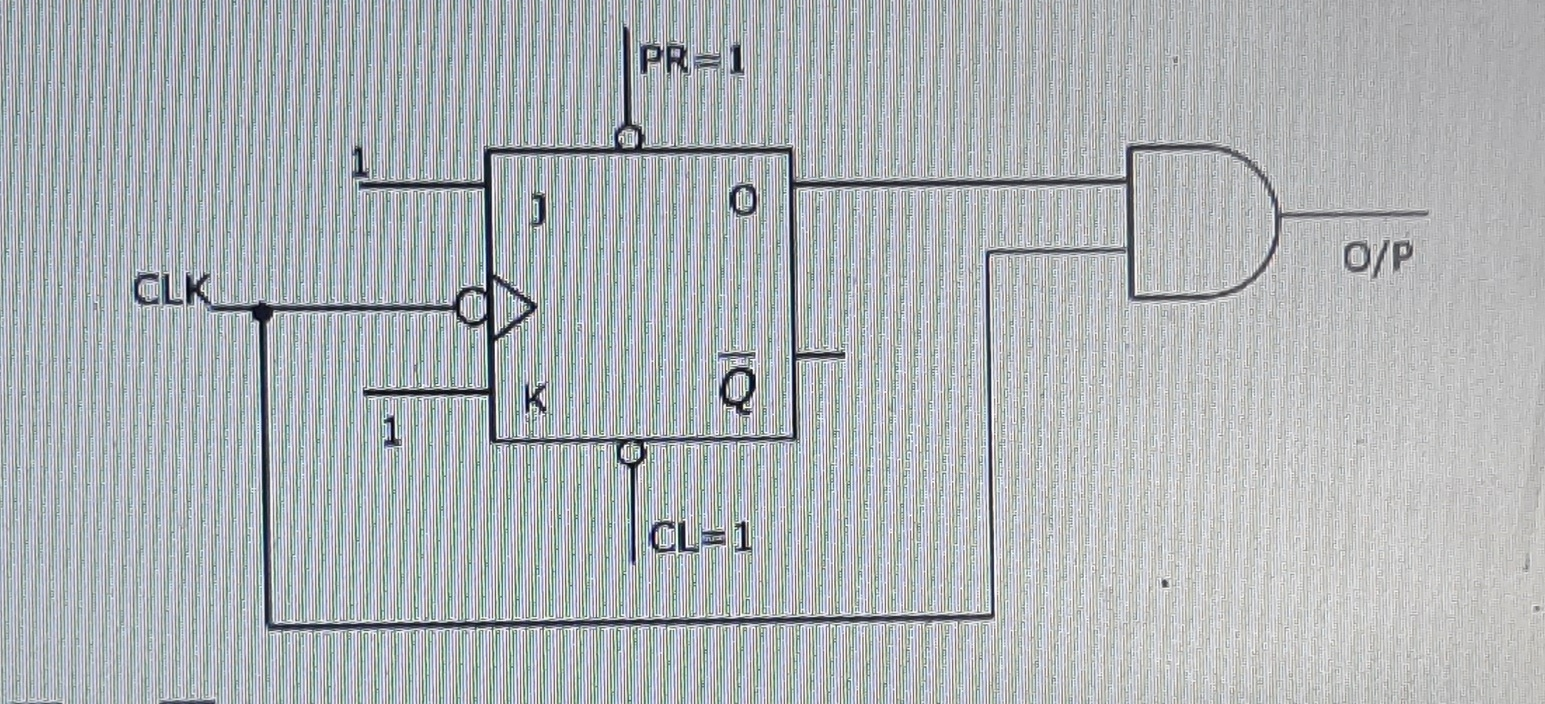
\includegraphics[width=0.75\columnwidth]{figs/2004-gate-ee-68.jpg}
	\caption{}
\label{fig:2004-gate-ee-68}
\end{figure}
\item The circuit shown in 
\figref{fig:2019-gate-in-12}
below uses ideal positive edge-triggered synchronous J-K flip flops with outputs X and Y. If the initial state of the output is X=0 and Y=0, just before the arrival of the first clock pulse, the state of the output just before the arrival of the second clock pulse is
\label{prob:2019-gate-in-12}
\hfill (GATE IN 2019)
\begin{figure}[H]
	\centering
	    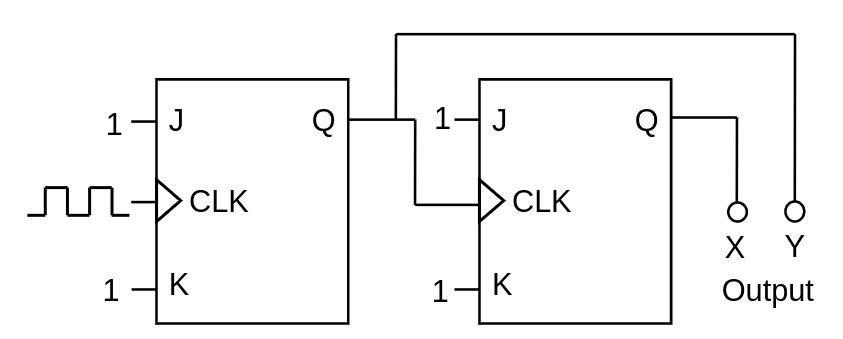
\includegraphics[width=0.75\columnwidth]{figs/2019-gate-in-12.png}
\caption{}
\label{fig:2019-gate-in-12}
\end{figure}
	\item 		
		A counter is constructed with three D flip-flops. The input-output pairs are named (D0, Q0), (D1, Q1), and (D2, Q2), where the subscript 0 denotes the least significant bit. The output sequence is desired to be the Gray-code sequence 000, 001, 011, 010, 110, 111, 101, and 100, repeating periodically. Note that the bits are listed in the Q2 Q1 Q0 format. Find the combinational logic expression for D1.
\label{prob:2021-gate-ee-37}
\hfill (GATE EE 2021)
\iffalse
\item The propogation delay of the exclusive-OR(XOR) gate in the circuit in Fig.
\label{prob:2021-gate-ec-46}
\ref{fig:2021-gate-ec-46}
is 3ns. The propogation delay of all the flip-flops is assumed to be zero. The clock(Clk) frequency provided to the circuit is 500MHz.
\begin{figure}[H]
\begin{center}
\resizebox{0.5\columnwidth}{!}{
\begin{tikzpicture}
\ctikzset{                                   
logic ports=ieee,                   
logic ports/scale=0.5               
}                                    
\draw(-1.3,0)node[xor port,anchor=out](x) {};         
\tikzstyle{dff}=[rectangle,draw,minimum height=7em,text width=7em,inner sep=3em]                                       
\node[dff] (dff2) {D2};                             
\node[dff, right=2cm of dff2] (dff1) {D1};           
\node[dff, right=2cm of dff1] (dff0) {D0};        
%Connecting flip-flops together                    
\draw (dff2.out) -- ++(2,0) node[above]{};        
\draw (dff1.out) -- ++(2,0) node[above] {};         
\draw (dff0.out) -- ++(2,0) node[above]{};          
\draw(dff2.out) -| (2.3,1.5) node[above]{$Q2$};        
\draw(dff1.out) -|(6.8,1.2) node[above]{$Q1$};         
\draw(dff0.out) -|(12.4,2) node[above]{$Q0$};          
\draw(x.in 2) -|(-3,2)to[short] (12.4,2);              
\draw(x.in 1)-|(-2.5,1.5)to[short](2.3,1.5);          
\draw(-2,-2) node[above]{$Clk$} --(6,-2);            
\draw(6,-2) node[above]{} --(9.1,-2);                 
\draw(9.1,-2)--(9.1,-1.2) node[above]{};                 
\draw(8.9,-1.23)--(9.1,-1)--(9.3,-1.23);               
\draw(4.5,-2)--(4.5,-1.2) node[above]{};               
\draw(4.3,-1.23)--(4.5,-1)--(4.7,-1.23);            
\draw(0,-2)--(0,-1.2) node[above]{};               
\draw(-0.2,-1.23)--(0,-1)--(0.2,-1.23);
\end{tikzpicture}

}
\end{center}
	\caption{Circuit}
\label{fig:2021-gate-ec-46}
\end{figure}
%
Starting from the initial value of the flip-flop outputs $Q2Q1Q0 =111$ with $D2=1$,the minimum number of triggering clock edges after which the flip-flop outputs $Q2Q1Q0$ becomes 1 0 0\emph{(in integer)} is \line(1,0){12.5}
\hfill (GATE EC 2021)
\fi
\item 
\label{prob:2022-gate-ec-43}
	 For the circuit shown in  
\figref{fig:2022-gate-ec-43},
		the clock frequency is $f_0$ and the duty cycle is $25 \%$. For the signal at the $Q$ output of the Flip-Flop,
\begin{enumerate}
	\item frequency of $\frac{f_0}{4}$ and duty cycle is 50$\%$
	\item frequency of $\frac{f_0}{4}$ and duty cycle is 25$\%$
	\item frequency of $\frac{f_0}{2}$ and duty cycle is 50$\%$
	\item frequency of $f_0$ and duty cycle is 25$\%$ \\
\end{enumerate}
\begin{figure}[H]
	\centering
    \resizebox{0.75\columnwidth}{!}{%
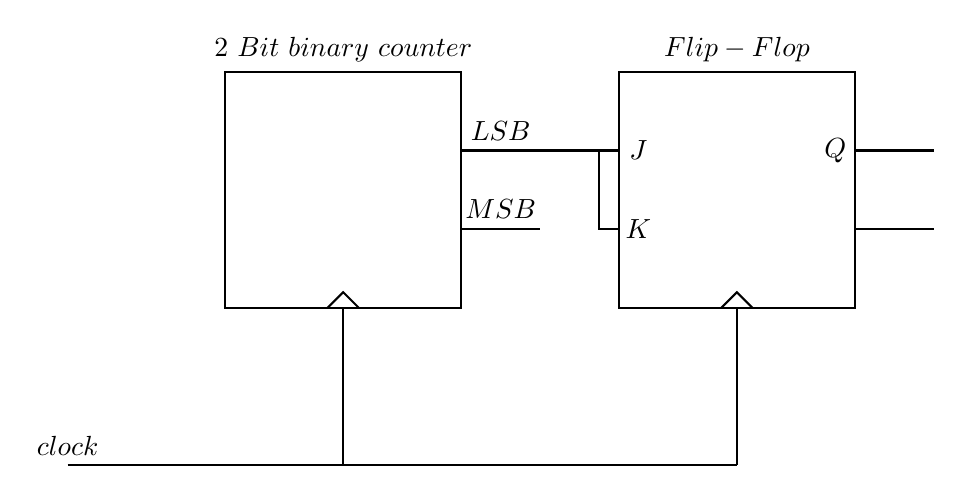
\begin{tikzpicture}
    \draw (2,2) rectangle (5,5);
    \draw (3.5,5) node[above]{$2$ $Bit$ $binary$ $counter$};
    \draw (3.3,2) -- (3.5,2.2) -- (3.7,2);
    \draw (7,2) rectangle (10,5);
    \draw (8.5,5) node[above]{$Flip-Flop$};
    \draw (8.3,2) -- (8.5,2.2) -- (8.7,2);
    \draw (5,3) -- (5.5,3) node[above]{$MSB$} -- (6,3);
    \draw (7.25,3) node{$K$};
    \draw (5,4) -- (5.5,4) node[above]{$LSB$} -- (7,4);
    \draw (7.25,4) node{$J$};
    \draw (6.75,4) -- (6.75,3) -- (7,3);
    \draw (0,0) node[above]{$clock$} -- (8.5,0);
    \draw (3.5,0) -- (3.5,2);
    \draw (8.5,0) -- (8.5,2);
    \draw (10,3) -- (11,3);
    \draw (9.75,4) node{$Q$} (10,4) -- (11,4);
\end{tikzpicture}

	}
	\caption{}
\label{fig:2022-gate-ec-43}
\end{figure}
\hfill 	(GATE EC-2022)
\item 
 Two T-flip flops are interconnected as shown in \figref{fig:tff1}. The present state of the flip flops are: $A = 1, B = 1$. The input x is given as $1, 0, 1$ in the next three clock cycles. The decimal equivalent of $(ABy)_{2}$ with A being the MSB and y being the LSB, after the 3\textsuperscript{rd} clock cycle is \rule{12mm}{0.4pt}
%
	\begin{figure}[H]
    \centering
    \resizebox{0.75\columnwidth}{!}{%
		\begin{tikzpicture}
  \draw (0,0) rectangle (2,3);

  \draw (-4,2.25) -- (0,2.25);
  \draw (-0.5,0.75) -- (0,0.75);
  \node[left] at (0.75,2.25) {$T_B$};
  \node[left] at (1.1,0.75) {$clk$};

  \draw (2,2.25) -- (4,2.25);
  \node[left] at (2,2.25) {$B$};
  

  \draw (0,0.4) -- (0.4,0.75) -- (0,1.1);

  \draw (0,4) rectangle (2,7);
  
  \draw (-0.5,6.25) -- (0,6.25);
  \draw (-0.5,4.75) -- (0,4.75);
  \node[left] at (0.75,6.25) {$T_A$};
  \node[left] at (1.1,4.75) {$clk$};

  \draw (-1.5,6.25) node[nand port] (nand) {};
  \draw (-4.5,6.525) -- (nand.in 1);
  \node[left] at (-4.5,6.525) {$x$};
  \draw (-2.9,3.5) -- (nand.in 2) ;
  \draw (nand.out) -- (-0.5,6.25) ;
  \draw (-4,2.25) -- (-4,6.525) ;
  \draw (-2.9,3.5) -- (3.5,3.5) ;
  \draw (3.5,3.5) -- (3.5,2.25) ;
  \filldraw (3.5,2.25) circle (2pt) ;
  \filldraw (-4,6.525) circle (2pt) ;
  \filldraw (-0.5,0.75) circle (2pt);

  \draw (5.5,5.965) node[or port] (or) {};
  \draw (4,6.25) -- (or.in 1) ;
  \draw (4,2.25) -- (4,5.685) ;
  \draw (4,5.685) -- (or.in 2) ;
  \node[right] at (or.out) {$y$} ;
  \draw (-0.5,4.75) -- (-0.5,-1.) ;
  \node[below] at (-0.5,-1.) {$clk$};
  
  \draw (2,6.25) -- (4,6.25);
  \node[left] at (2,6.25) {$A$};

  \draw (0,4.4) -- (0.4,4.75) -- (0,5.1);
  
\end{tikzpicture}
		}
		\caption{}
		\label{fig:tff1}
	\end{figure}
		\hfill (GATE IN 2020)
% Two T-flip flops are interconnected as shown in \figref{fig:tff1}. The present state of the flip flops are: $A = 1, B = 1$. The input x is given as $1, 0, 1$ in the next three clock cycles. The decimal equivalent of $(ABy)_{2}$ with A being the MSB and y being the LSB, after the 3\textsuperscript{rd} clock cycle is \rule{12mm}{0.4pt}

		\vspace{1cm}
	\begin{figure}[ht]
		\centering
		\begin{tikzpicture}
  \draw (0,0) rectangle (2,3);

  \draw (-4,2.25) -- (0,2.25);
  \draw (-0.5,0.75) -- (0,0.75);
  \node[left] at (0.75,2.25) {$T_B$};
  \node[left] at (1.1,0.75) {$clk$};

  \draw (2,2.25) -- (4,2.25);
  \node[left] at (2,2.25) {$B$};
  

  \draw (0,0.4) -- (0.4,0.75) -- (0,1.1);

  \draw (0,4) rectangle (2,7);
  
  \draw (-0.5,6.25) -- (0,6.25);
  \draw (-0.5,4.75) -- (0,4.75);
  \node[left] at (0.75,6.25) {$T_A$};
  \node[left] at (1.1,4.75) {$clk$};

  \draw (-1.5,6.25) node[nand port] (nand) {};
  \draw (-4.5,6.525) -- (nand.in 1);
  \node[left] at (-4.5,6.525) {$x$};
  \draw (-2.9,3.5) -- (nand.in 2) ;
  \draw (nand.out) -- (-0.5,6.25) ;
  \draw (-4,2.25) -- (-4,6.525) ;
  \draw (-2.9,3.5) -- (3.5,3.5) ;
  \draw (3.5,3.5) -- (3.5,2.25) ;
  \filldraw (3.5,2.25) circle (2pt) ;
  \filldraw (-4,6.525) circle (2pt) ;
  \filldraw (-0.5,0.75) circle (2pt);

  \draw (5.5,5.965) node[or port] (or) {};
  \draw (4,6.25) -- (or.in 1) ;
  \draw (4,2.25) -- (4,5.685) ;
  \draw (4,5.685) -- (or.in 2) ;
  \node[right] at (or.out) {$y$} ;
  \draw (-0.5,4.75) -- (-0.5,-1.) ;
  \node[below] at (-0.5,-1.) {$clk$};
  
  \draw (2,6.25) -- (4,6.25);
  \node[left] at (2,6.25) {$A$};

  \draw (0,4.4) -- (0.4,4.75) -- (0,5.1);
  
\end{tikzpicture}
		\caption{}
		\label{fig:tff1}
		\hfill (GATE IN 2020)
	\end{figure}

\item In the circuit shown below in \figref{fig:image} a positive edge-triggered D flip-flop is used for sampling input data
 using clock CK.The XOR gate outputs 3.3 volts for logic HIGH and 0 volts for logic LOW levels.
The data bit and clock periods are equal and the value of $ \Delta T / T_{ck} $ = 0.15,where
the parameters $ \Delta T $ and $ T_ck$ are shown in the figure.Assume  that the Flip and
the XOR gate are ideal.  
\begin{figure*}[!ht] 
	\centering
    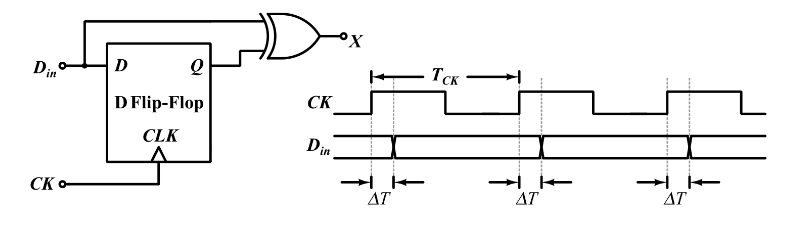
\includegraphics[width=0.75\columnwidth]{figs/image.png} 
    \caption{}
    \label{fig:image}
 \end{figure*}
\label{fig:2018-gate-ec-46}

\hfill(GATE EC 2018)
\item A 2-bit synchronous counter using two J-K flip flops is shown
	in \figref{fig:enter-label}.
 The expressions for the inputs to the J-K flip flops are also shown in the figure. The output sequence of the counter starting from $Q_1Q_2 = 00$ is 
\begin{figure}[H]
	\centering
	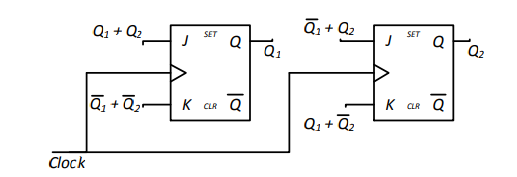
\includegraphics[width=0.75\columnwidth]{figs/question44.png}
	\caption{}
	\label{fig:enter-label}
\end{figure}
\begin{enumerate}
	\item $00\rightarrow11\rightarrow10\rightarrow01\rightarrow00...$ 
        \item $00\rightarrow01\rightarrow10\rightarrow11\rightarrow00...$
        \item $00\rightarrow01\rightarrow11\rightarrow10\rightarrow00...$
        \item $00\rightarrow10\rightarrow11\rightarrow01\rightarrow00...$
\end{enumerate}
\hfill{GATE IN 2018}
\item A $16$-bit synchronous binary up-counter is clocked with the frequency $\vec{f}_{\text{CLK}}$. The two most significant bits are $\vec{OR}$-ed together to form an output $Y$. Measurements show that $Y$ is periodic, and the duration for which $Y$ remains high in each period is $24$ ms. The clock frequency\underline{\hspace{2cm}}MHz.\\ {(Round off to $2$ decimal places.)}
\hfill{\brak{GATE \enspace EE2021-22}}

\item The sequence of states ($Q_1Q_0$) of the given synchronous sequential circuit is \makebox[4em]{\hrulefill}.

\hfill{\brak{GATE \enspace EC2024}}

\tikzset{every picture/.style={line width=0.75pt}} %set default line width to 0.75pt        

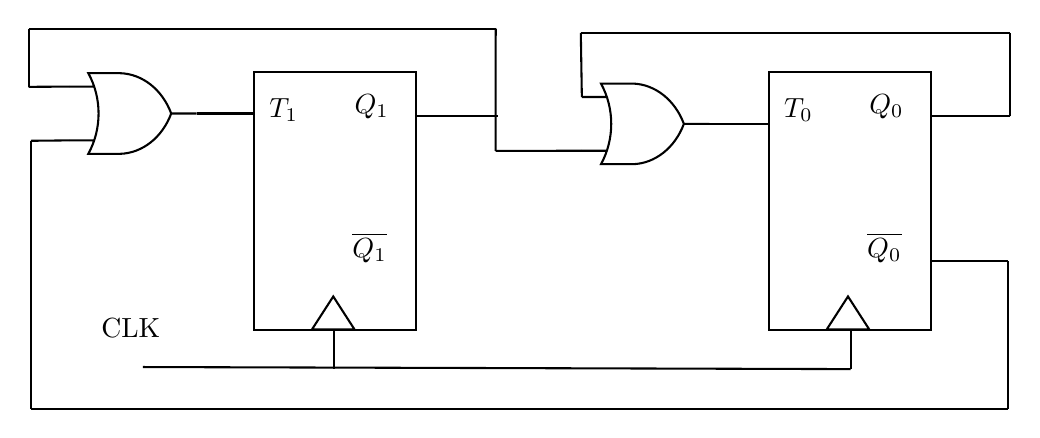
\begin{tikzpicture}[x=0.75pt,y=0.75pt,yscale=-1,xscale=1]
%uncomment if require: \path (0,300); %set diagram left start at 0, and has height of 300

%Shape: Rectangle [id:dp8202540055907639] 
\draw   (158,53) -- (236,53) -- (236,177) -- (158,177) -- cycle ;
%Shape: Or Gate [id:dp08978132180586507] 
\draw   (78.22,53.43) -- (93.58,53.43) .. controls (104.3,53.77) and (113.88,61.34) .. (118.16,72.85) .. controls (113.88,84.36) and (104.3,91.93) .. (93.58,92.28) -- (78.22,92.28) .. controls (84.8,80.25) and (84.8,65.45) .. (78.22,53.43) -- cycle (69,59.9) -- (81.29,59.9) (69,85.8) -- (81.29,85.8) (118.16,72.85) -- (130.45,72.85) ;
%Shape: Triangle [id:dp8379215440652463] 
\draw   (196.23,161) -- (206.45,176.85) -- (186,176.85) -- cycle ;
%Shape: Rectangle [id:dp5064333177931405] 
\draw   (406,53) -- (484,53) -- (484,177) -- (406,177) -- cycle ;
%Shape: Triangle [id:dp04508106309695603] 
\draw   (444.23,161) -- (454.45,176.85) -- (434,176.85) -- cycle ;
%Straight Lines [id:da8430836438701459] 
\draw    (130.45,72.85) -- (158.45,72.85) ;
%Shape: Or Gate [id:dp27911316649955176] 
\draw   (325.22,58.43) -- (340.58,58.43) .. controls (351.3,58.77) and (360.88,66.34) .. (365.16,77.85) .. controls (360.88,89.36) and (351.3,96.93) .. (340.58,97.28) -- (325.22,97.28) .. controls (331.8,85.25) and (331.8,70.45) .. (325.22,58.43) -- cycle (316,64.9) -- (328.29,64.9) (316,90.8) -- (328.29,90.8) (365.16,77.85) -- (377.45,77.85) ;
%Straight Lines [id:da7800420433441013] 
\draw    (377.45,77.85) -- (405.45,77.85) ;
%Straight Lines [id:da7788178738488024] 
\draw    (274.45,90.85) -- (316,90.8) ;
%Straight Lines [id:da39345195977505776] 
\draw    (235.5,74) -- (275.5,74) ;
%Straight Lines [id:da6068351001271327] 
\draw    (274.5,32) -- (274.45,90.85) ;
%Straight Lines [id:da18722802985553144] 
\draw    (49.5,32) -- (274.5,32) ;
%Straight Lines [id:da5744513622437428] 
\draw    (49.5,32) -- (49.5,60) ;
%Straight Lines [id:da80433220708581] 
\draw    (69,59.9) -- (49.5,60) ;
%Straight Lines [id:da6540890230403057] 
\draw    (521.5,144) -- (484.5,144) ;
%Straight Lines [id:da10980162685426853] 
\draw    (521.5,215) -- (521.5,144) ;
%Straight Lines [id:da6573970266628919] 
\draw    (50.5,215) -- (521.5,215) ;
%Straight Lines [id:da8030222177883335] 
\draw    (50.5,215) -- (50.5,86) ;
%Straight Lines [id:da4832475128489785] 
\draw    (50.5,86) -- (69,85.8) ;
%Straight Lines [id:da043356258414056326] 
\draw    (316,64.9) -- (315.5,34) ;
%Straight Lines [id:da6906606003899586] 
\draw    (522.5,34) -- (315.5,34) ;
%Straight Lines [id:da13292875849313357] 
\draw    (522.5,34) -- (522.5,74) ;
%Straight Lines [id:da8943203868157404] 
\draw    (522.5,74) -- (484.5,74) ;
%Straight Lines [id:da13168982284438902] 
\draw    (104.5,195) -- (445.5,196) ;
%Straight Lines [id:da18651973646229014] 
\draw    (196.5,177) -- (196.5,196) ;
%Straight Lines [id:da9854734273448209] 
\draw    (445.5,177) -- (445.5,196) ;

% Text Node
\draw (164,64) node [anchor=north west][inner sep=0.75pt]   [align=left] {$\displaystyle T_{1}$};
% Text Node
\draw (205,62) node [anchor=north west][inner sep=0.75pt]   [align=left] {$\displaystyle Q_{1}$};
% Text Node
\draw (204,129) node [anchor=north west][inner sep=0.75pt]   [align=left] {$\displaystyle \overline{Q_{1}}$};
% Text Node
\draw (412,64) node [anchor=north west][inner sep=0.75pt]   [align=left] {$\displaystyle T_{0}$};
% Text Node
\draw (453,62) node [anchor=north west][inner sep=0.75pt]   [align=left] {$\displaystyle Q_{0}$};
% Text Node
\draw (452,129) node [anchor=north west][inner sep=0.75pt]   [align=left] {$\displaystyle \overline{Q_{0}}$};
% Text Node
\draw (83,170) node [anchor=north west][inner sep=0.75pt]   [align=left] {CLK};


\end{tikzpicture}


\begin{enumerate}[label=(\Alph*)]
    \item 00 $\to$ 10 $\to$ 11 $\to$ 00
    \item 11 $\to$ 00 $\to$ 10 $\to$ 01 $\to$ 00
    \item 01 $\to$ 10 $\to$ 11 $\to$ 00 $\to$ 01
    \item 00 $\to$ 01 $\to$ 10 $\to$ 00
\end{enumerate}


\end{enumerate}
